\documentclass[11pt, a4paper, titlepage]{article}
\usepackage[utf8]{inputenc}


%Margins
\usepackage[a4paper, total={6in, 9in}]{geometry}

%Català 
\usepackage[T1]{fontenc}
\usepackage[utf8]{inputenc}
%\usepackage[catalan]{babel}

%Imatges i peu de imatge
\usepackage{graphicx}
\usepackage{caption}
\usepackage{bmpsize}

\usepackage{amsmath}
\usepackage{ amssymb }
\usepackage{subcaption}
\usepackage{wrapfig}
\usepackage{adjustbox}

%Incloure codi
\usepackage{listings}

%Eliminar espai abans del primer item en itemize
\usepackage{enumitem}
\setlist{nolistsep}

%€
\usepackage[official]{eurosym}

%Links
\usepackage{hyperref}

%Colors
\usepackage{color}
\usepackage{enumitem}


\edef\restoreparindent{\parindent=\the\parindent\relax}
\usepackage[parfill]{parskip}
\restoreparindent
\hypersetup{%
    pdfborder = {0 0 0}
}


\usepackage{bibentry}



\title{\textbf{{\Large Data Analysis and Knowledge discovery} \\ - \\ Data visualization analysis on American comics characters}}
\author{Laura C.}
\date{16 of January, 2018}

\begin{document}

\maketitle

\tableofcontents

\newpage
\section{Introduction}
Nowadays, american comics have been established as a hobby for many, apparently regardless of the consumer's age or gender. They are a form of entertainment which has settled despite the virtual era taking place, maybe due to the fidelity of its consumers.


\noindent\begin{minipage}{0.3\textwidth}% adapt widths of minipages to your needs

\includegraphics[width=\linewidth]{img/marvel_logo.png}
\end{minipage}%
\begin{minipage}{0.02\textwidth}%\raggedleft
\hfill%

\end{minipage}
\begin{minipage}{0.68\textwidth}%\raggedleft

\textit{Marvel Comics} is a company now owned by \textit{The Walt Disney Company} founded at 1939 in the United States of America, under the name of \textit{Timely Comics} and after changing its name two times it has established itself as one of the two giants that produce occidental comics.


Its most popular characters are the classical superheroes that most people world wide know about: \textit{Spider-man, Wolverine, the Hulk, Thor, Iron Man and Captain America}.
\end{minipage}


\begin{minipage}{0.78\textwidth}% adapt widths of minipages to your needs

The other giant and main competitor of \textit{Marvel Comics} is \textit{DC Comics}, which was founded at the United States of America in 1934 under the name of \textit{National Allied Publications}. It is now owned by \textit{Disney}'s competitor, the \textit{Warner Bros} company.

\textit{DC Comics} most popular characters are \textit{Superman, Batman, Wonder Woman, Green Lantern and The Flash}, among many others.  
\end{minipage}%
\begin{minipage}{0.02\textwidth}%\raggedleft
\hfill%

\end{minipage}
\begin{minipage}{0.2\textwidth}%\raggedleft

\includegraphics[width=\linewidth]{img/DC_Comics_logo.png}
\end{minipage}



Now, if we took a closer look on the examples we have given about each company we will notice that only one woman is among all of them, being the rest all men. 

The aim of this project is to study the american comic characters of the companies \textit{Marvel} and \textit{DC Comics} to see if each one of them and the hobby altogether tends to produce a specific, stereotyped and biased character. This bias being that there is dependency between different attributes of a character, instead of trying to produce characters of different types in all aspects.

\newpage
\section{About the dataset}
The dataset
\footnote{https://github.com/fivethirtyeight/data/tree/master/comic-characters} has been obtained by \textit{FiveThirtyEight}, a website focused on politics, economics, sports and opinion polls analysis.\footnote{https://en.wikipedia.org/wiki/FiveThirtyEight}

The data was scrapped from the respective fans encyclopedias (commonly known as \textit{Wikias}) of \textit{Marvel} and \textit{DC Comics} in 2013. So new data from 2013 onwards is missing.

\begin{center}
  \begin{tabular}{lr}
\textbf{Company} & \textbf{\# Individuals} \\ \hline
Marvel & 16376 \\
DC & 6896 \\
\textbf{Total} & \textbf{23253}
\end{tabular}
\end{center}

The dataset's script  to obtain updated data, which is not available, scrapped the following aspects:
\begin{itemize}
  \item \textbf{Page id} from where the character's data was scrapped.
  \item \textbf{Character's name}.
  \item \textbf{URL suffix}.
  \item \textbf{Characters' identity status} in its world.
    \begin{itemize}
      \item Secret
      \item Public
      \item Not a dual entity
    \end{itemize}
  \item \textbf{Alignment}. Whether the character is a superhero or an antagonist. It is reduced to:
    \begin{itemize}
      \item Good.
      \item Bad.
      \item Neutral.
      \item Reformed criminal.
    \end{itemize}
  \item \textbf{Eyes' color}. A variety of 18 colors.
  \item \textbf{Hair's color}. A variety of 20 colors.
  \item \textbf{Gender}, which can be:
    \begin{itemize}
      \item Female
      \item Male
      \item Genderless
      \item Transgender
    \end{itemize}
  \item \textbf{GSM:} Whether the character sexuality is:
  \begin{itemize}
    \item Bisexual
    \item Homosexual
    \item Transgender
    \item Transvestite
    \item Genderfluid
    \item Pansexual
    \item Heterosexual or unspecified.
  \end{itemize}
  \item \textbf{Living status.} The character is either dead of alive.
  \item \textbf{Total number of appearances} in the comics.
  \item \textbf{Year of first appearance}.
\end{itemize}

\textbf{Notice that the data is qualitative but not quantitative or linear}. This has been chosen in purpose in order to study (albeit if only briefly) how to be able to explore non numerical data, which is often the only type of data studied in the different courses in this masters programe.

\section{Goals}

This project is threefold:
\begin{enumerate}
  \item \textbf{Clean the data} and check how the cleaning affects the size of the dataset. That is, check the quality of the dataset and improve it when possible.\\
  \item \textbf{Explore the dataset} by studying the different relationships between variables of characters in american comic books. Those relationships being:
    \begin{itemize}
    \item Genders'
    \begin{itemize}
      \item General ratio.
      \item Appearance throughout the years.
    \end{itemize}
  
    \item Ratio of alive/dead.
    \item Correlation between the alignment taken and the gender.\\
    
  \end{itemize}
 \item \textbf{Study possibles structures in the dataset} formed by different variables. For this, we have chosen Multiple Correspondence Analysis as a method to explore our qualitative data.\\
\end{enumerate}

Both the code and datasets can be found attached to this report.

The exploration of the dataset will be conducted in both a \textbf{general dataset} conformed by the characters of the two companies and a \textbf{subset} of it, formed by the characters that have appeared most times in their respective series. Because of the times they have appeared we will assume them to be also the \textbf{most popular characters}.

\newpage
\section{Data cleaning}

Before starting to explore and study the data, we should start cleaning the datasets and get familiar to the dataset to know what should stay and what should be removed.

\subsection{Dataset analysis}

We have a total of 13 variables and we can see that except for the year of first appearance and number of appearances throughout the years, the data is not numerical. This means that we cannot work using correlations matrices or well-known methods such as ANOVA, \textbf{Principal Component Analysis}  (PCA) or \textbf{Linear Discriminant Analysis} (LDA) on it, for they require the data to be numerical.

Is for this reason that since the data is qualitative that we should apply \textbf{Multiple Correspondence Analysis} (MCA).

On the other hand, the characters of Marvel and DC are split in two different files (each compiling the characters of one company) with identical columns. Since this study is performed on both groups of characters in their totality, we will have to join them.

In addition, we are only interested in the character's names, identity status, alignment, eye and hair colors, gender, sexuality, living status, the number of appearances and the year of the first one, meaning that some columns are redundant or uninteresting for this study.
 
 Finally, observing the data it can be seen that often fields are void in many cases. That is the case, for example, of GSM. When it is empty it means that the characters do not form part of a minority group. In this case, the void to be filled is interpretable. However, the same rule of assumption cannot be applied to the character's alignment, so characters that are not positioned should not be taken into account in our study.
  

\subsection{Steps}
From the analysis, we have determined and applied the following steps to clean the data:

 \begin{enumerate}
   \item Joined the files into one big dataset to work with,  instead of two in parallel.
      \item Removed the columns of data of variables we are not interested in. That is, removed the page id, the URL suffix and the first appearance specified in "year, month" format.
      \item Filled the voids when possible. That is, filled the voids that are interpretable. That is the case of GSM.
   \item Removing rows when the void fields are impossible to fill and thus untreatable. This is the case for characters with no alignment, eye color, hair color, gender and living status.  
   \item Some categories were repetitive, such as repeating the word \textit{Characters} on the gender field. These words have been removed to enforce clarity and avoid redundancy on future graphics.
 \end{enumerate}
 

 Before cleaning the data, we had 23253 characters, 16376 of which are from Marvel and 6896 from DC. 
 
 After removing rows where the character had no value for its gender, alive or not and alignment, the dataset resulted in 6799 rows.  From those, 4692 are from Marvel and 2107 from DC Comics.
 
 Which means that a total of 16454 comic characters had no fillable variables and we will be working with only the 29.23\% of the characters from the original dataset.

\begin{figure}[!htb]
    \centering
    \begin{minipage}{.5\textwidth}
        \centering
        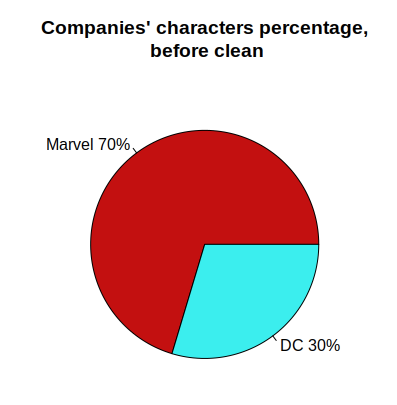
\includegraphics[width=.8\linewidth]{img/pie_bf_company.png}
    \end{minipage}%
    \begin{minipage}{0.5\textwidth}
        \centering
        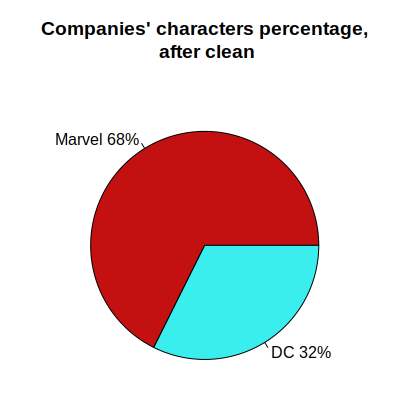
\includegraphics[width=0.8\linewidth]{img/pie_after_comp.png}
    \end{minipage}
\end{figure}

With this we can see that Marvel dataset was more incomplete than DC one, although both had a lot of missing data which resulted in less than a third of the original data. However, this reduction is justified by wanting to see relationships between different data. Were a category be missing for a characteristic, then MCA could not be applied.


Additionally, a\textbf{ subset of this one has been made} in order to be able to work with MCA. It is conformed by the characters that have appeared most times, and the criteria and need of this subset has been explained in detail in the MCA section. It will be referred to as the most popular characters and its usage will be explicit in this report. 

\textbf{When no specification of which dataset is used has been made in the report, it is assumed that we are working on the general one.}


\newpage
\section{Study}
Having cleaned the data now we can study it adequately by checking relationships the variables and the characteristics of the variables themselves.

\subsection{Simple analysis}
Before proceeding on applying MCA to the dataset we are going to check the different variables individually (or related to a couple of others).

\subsubsection{Characters' gender}
A plot has been made where the characters gender can be seen.

\begin{figure}[!htb]
    \centering
    \begin{minipage}{.43\textwidth}
        \centering
        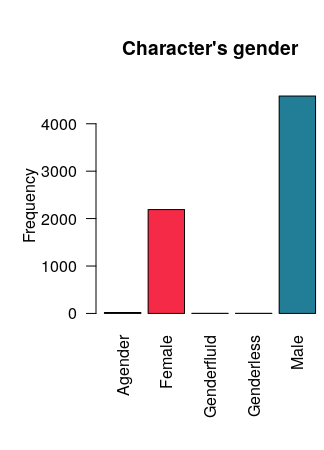
\includegraphics[width=\linewidth]{img/genders_plot.png}
    \end{minipage}%
     \begin{minipage}{.10\textwidth}
      \hfill
    \end{minipage}%
    \begin{minipage}{0.47\textwidth}
      \centering
        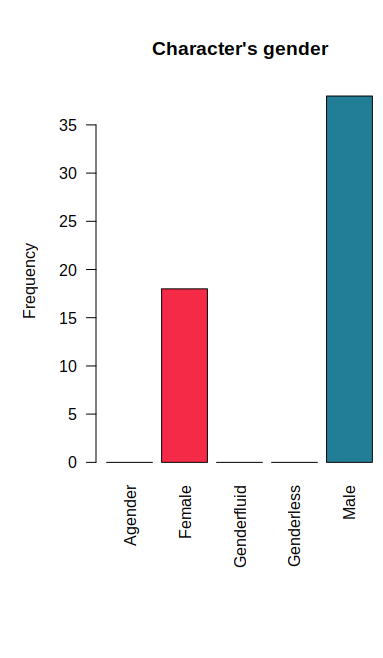
\includegraphics[width=\linewidth]{img/genders_plot_pop.png}
    \end{minipage}
\end{figure}


  Notice that there are mainly male characters in both the general dataset and the popular one, followed (by a large margin) by female ones. 
  
       However, this just indicates that there have been more than twice times more males than females without taking into account their number of occurrences in the series nor when they first appeared.
       
       We can also see that some agender and genderless characters exist in the general dataset, as well as genderfluid ones. But their numbers are not as meaningful as their counterparts and cannot compare to them. 
       
So to be able to compare them more precisely, we can check this table, where the total number of counts as well as the percentage in relation to the total number of characters is shown.

The fact that the ratio mantains when working with a subset of the main characters nonetheless just demonstrates further that there the comics are male dominant.

\begin{center}

\begin{tabular*}{0.4\textwidth}{l@{\extracolsep{\fill}}rr}
 & \multicolumn{1}{c}{\textbf{Counts}} & \multicolumn{1}{c}{\textbf{\%}} \\ \hline
\textbf{Agender} & 19 & 0,279 \\
\textbf{Female} & 2190 & 32,210 \\
\textbf{Genderfluid} & 2 & 0,029 \\
\textbf{Genderless} & 3 & 0,0441\\
\textbf{Male} & 4585 & 67,436 \\ \hline \hline
\textbf{Total} & \textbf{6799} & \textbf{100}
\end{tabular*}

\end{center}

A boxplot has been made for each gender:

\begin{center}
   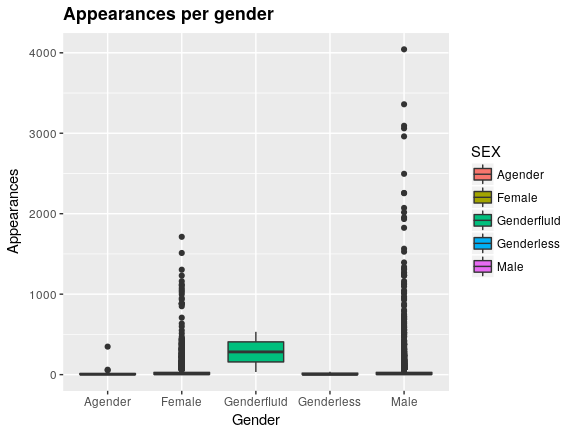
\includegraphics[width=0.8\linewidth]{img/appearances_per_gender.png}
\end{center}
Although only a boxplot is created for the genderfluid characters, meaning that the tree genderlfuid characters appear more or less the same number of times.

For the rest of the characters, we can conclude that they do not appear a more or less uniform number of times, but instead there seems to be a lot of disparity on their number of appearances (as defined by the large number of outliers), which would mean only a minority of characters appear more than just once or twice. We can see this disparity again  in the plot below.
\begin{center}
   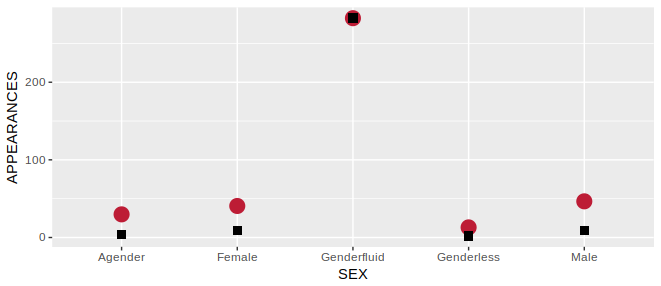
\includegraphics[width=0.6\linewidth]{img/mean_median.png}
\end{center}

The red dots represent the mean meanwhile the black squares represent the median. As we can see, in almost all genders (except the genderfluid were only three individuals are categorized as such) the median is well below the average, which means \textbf{there are several characters in each gender that appear way more times than others}, thus increasing the average. The median indicates us that, when ordered, at least half the population is below the average.


After seeing the number of appearances of each gender, now we'll focus on \textbf{when} they  were introduced and \textbf{how many} per gender.

For this, two more plots have been made to see the evolution of the number of characters produced by year and by gender.

\begin{center}
   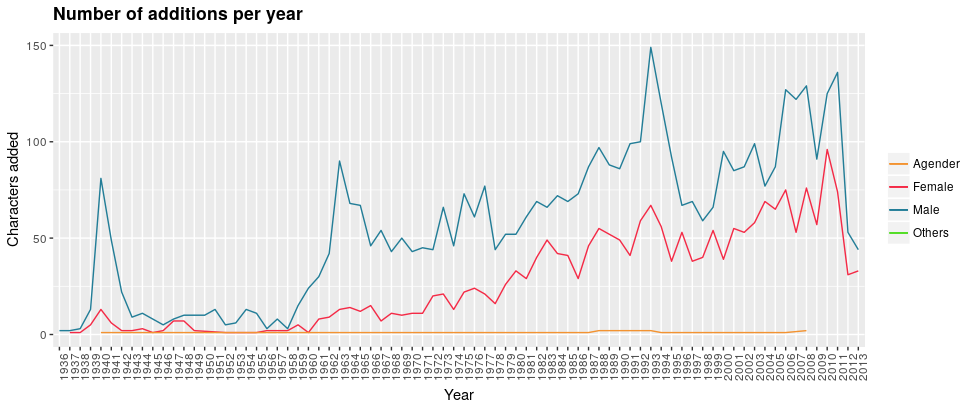
\includegraphics[width=\linewidth]{img/add_per_year.png}
 \end{center}
 \begin{center}
   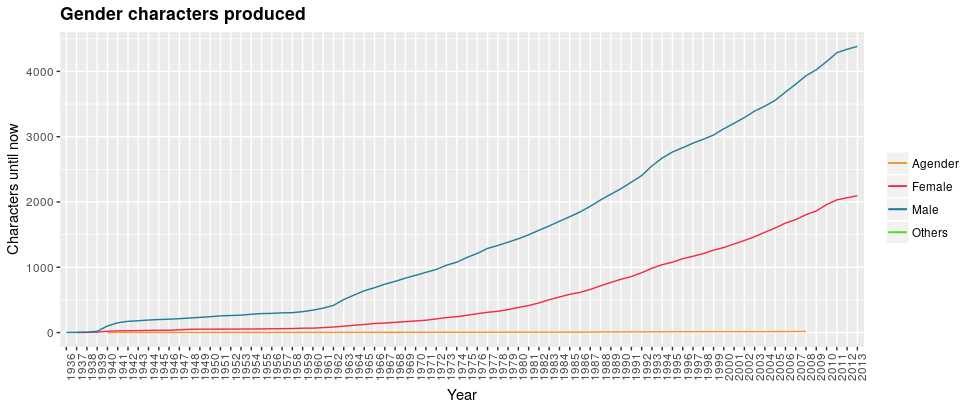
\includegraphics[width=\linewidth]{img/gender_char_prod.png}
\end{center}

We have treated the Agender and genderless as one group, and we can see that they have been introduced from the started but were not included again until on the 70's and 80's. The others (transgender and genderfluid)  only appeared starting the 70's, which unfortunately is not shown on the graphics directly because they have been overlapped by the agender group.

We can also see that on the later years, specially starting on 2010, they gap between male and female characters has been closing. But one should notice that there has never been a year were the leading gender group has not been a male character. Which enforces the idea of male predominant comic worlds.

\subsubsection{Living status}

As for the living status of the characters, we plot it for both the whole dataset and the one containing the most popular characters.

\begin{figure}[!htb]
    \centering
    \begin{minipage}{.47\textwidth}
        \centering
        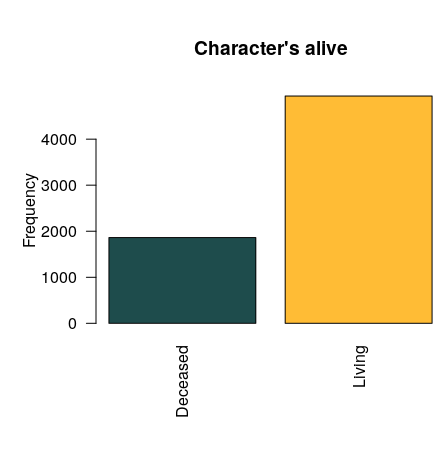
\includegraphics[width=\linewidth]{img/aliveratio.png}
        \captionof{figure}{Living status for whole dataset}
    \end{minipage}%
     \begin{minipage}{.06\textwidth}
      \hfill
    \end{minipage}%
    \begin{minipage}{0.47\textwidth}
       \centering
       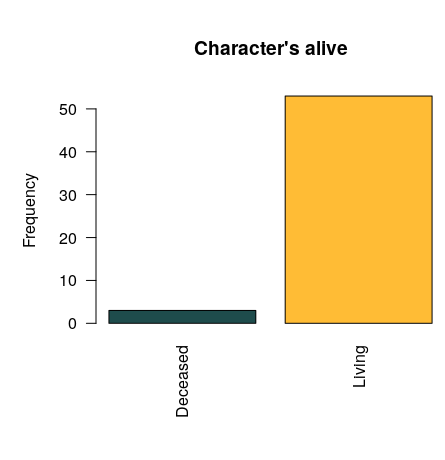
\includegraphics[width=\linewidth]{img/popdeceasedalive.png}
       \captionof{figure}{Living status for most popular chars.}
    \end{minipage}
\end{figure}

In the left we can see the plot for all characters. There are almost three times more living characters than dead ones. Whereas if we check those that are popular, we can see that most of them are alive.

So we can conclude there is reticence on killing characters that have appeared many times during the series.

It should also be told that no female character has died in the popular characters dataset, so every deceased is male.

\subsubsection{Alignment}
%% ALIGMENT
The alignment is the attribute that tells us whether the character is good, bad or neutral.

For the whole dataset the numbers are as follow:
\begin{center}
  
\begin{tabular*}{0.6\textwidth}{l@{\extracolsep{\fill}}ccc}
 & \textbf{Good} & \textbf{Bad} & \textbf{Neutral} \\ \hline
\textbf{Female} & 1192 & 579 & 419 \\
\textbf{Male} & 1835 & 2045 & 704\\
\end{tabular*}

\end{center}

Whereas for the main characters is:
\begin{center}
\begin{tabular*}{0.6\textwidth}{l@{\extracolsep{\fill}}ccc}
 & \textbf{Good} & \textbf{Bad} & \textbf{Neutral} \\ \hline
\textbf{Female} & 17 & 0 & 1 \\
\textbf{Male} & 32 & 0 & 6\\
\end{tabular*}
  
\end{center}

There are a couple of interesting things that can be seen just looking at the numbers:
\begin{enumerate}
  \item In the whole dataset, there are slightly more bad females than neutral, but the numbers are close.
  \item In the whole dataset, most girls are good.
  \item In the whole dataset, there are way noticeably more bad characters than good.
  \item No bad characters are present in the main characters subset. So the ones that appear the most are those either neutral or good.\\
\end{enumerate}

We can see these numbers plotted as follow:
\begin{center}
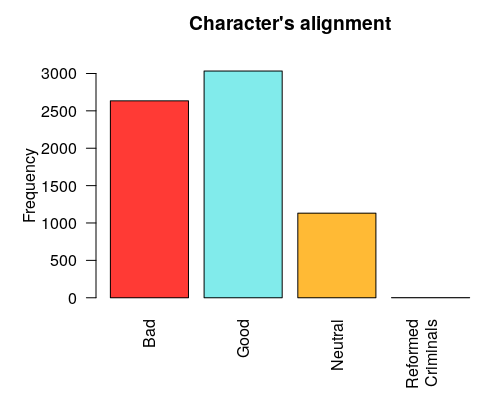
\includegraphics[width=0.4\linewidth]{img/alignment.png}
\end{center}
 
\begin{figure}[!htb]
    \centering
    \begin{minipage}{.47\textwidth}
        \centering
        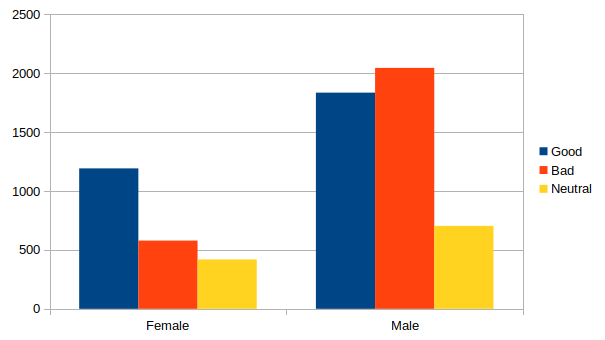
\includegraphics[width=\linewidth]{img/alignment_gender_total.png}
        \captionof{figure}{Align. whole dataset}
    \end{minipage}%
     \begin{minipage}{.06\textwidth}
      \hfill
    \end{minipage}%
    \begin{minipage}{0.52\textwidth}
       \centering
       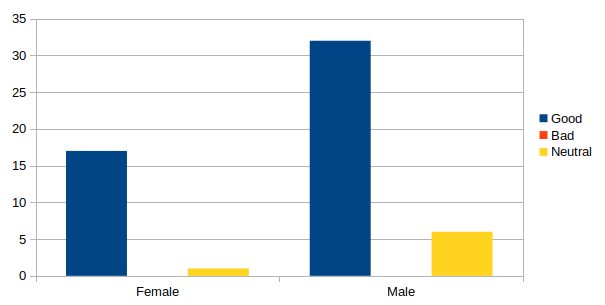
\includegraphics[width=\linewidth]{img/alignment_gender.png}
       \captionof{figure}{Align.  most popular chars.}
    \end{minipage}
\end{figure}

\newpage
\subsection{Multiple Correspondence Analysis}
This method, also known as \textbf{MCA}, is a technique in Data Analysis applied to data which is nominal categorical. That is, not numerical. It is used to detect and represent structures in a data set by showing each individual in the data set as a point in a low-dimensional Euclidean Space.

It is considered an extension of Correspondence Analysis, but applied (as its name indicates) to variables' categories that are large.

Its homologous on continuous data would be Principal Component Analysis.

\subsubsection{Explanation}
This method treats rows and columns equivalently, so an individual cannot have a field empty. It creates a factor score for each individual from weighting the rows and columns.
There are three phases to apply in MCA.
\begin{enumerate}
  \item \textbf{Preprocess the table} creating a contingency one of the same size: $ C = m *n$ where the weights for each cell is computed. The row weight is computed such that $w_{m} = \frac{1}{n_{C}} CV$ and the column weight such that: $w_{m} = \frac{1}{n_{C}} V^{T}_{1}C$., where each cell $n_{C} = \sum_{i=1}^{n} \sum_{j=1}^{m} C_{ij} $.\\ In other words, $w_{m}$ and $w_{n}$ compute the marginal probabilities of the rows and columns classes.\\

  $V_{1}$ is a column vector of 1 with the dimension of the column. \\
  
  Then it creates table $S$ where each cell of the table $C$ is divided by $n_{C}$, which is the total sum of $C$ table:
 $S = \frac{1}{n_{C}} C$\\
 
 This computes the joint probability distribution of the rows and columns.\\
 
 And finally, it creates table $M$ applying to the table $S$ the weights of each row and column computed previously:
 $M = S - w_{m}w_{n}$, which means that it computes the deviations from independence.
 
  \item  \textbf{Create orthogonal components} from the computed table $M$, where $M$ is decomposed applying the generalized singular value decomposition, resulting in $M = U\sum V^*$, where $U^W_{m}U = V^{*}W_{n}V = I$
  \item Compute the \textbf{factor scores} for both the row and columns items:
  $F_{m} = W_{m}U\sum$, $F_{n} = W_{n}V\sum$.
  
\end{enumerate}

Knowing how MCA works we can now proceed to apply it to our dataset to try to find underlying structures between variables' categories.


\subsubsection{MCA applied}
If we apply the method to the totality of our clean dataset (6799 individuals) it takes more than half an hour to produce a result. Furthermore, as we can see, there is no clear relationship between the characters' variables. By checking the X and Y axis, we can see that only 0.1\% of variability is explained.


\begin{center}
   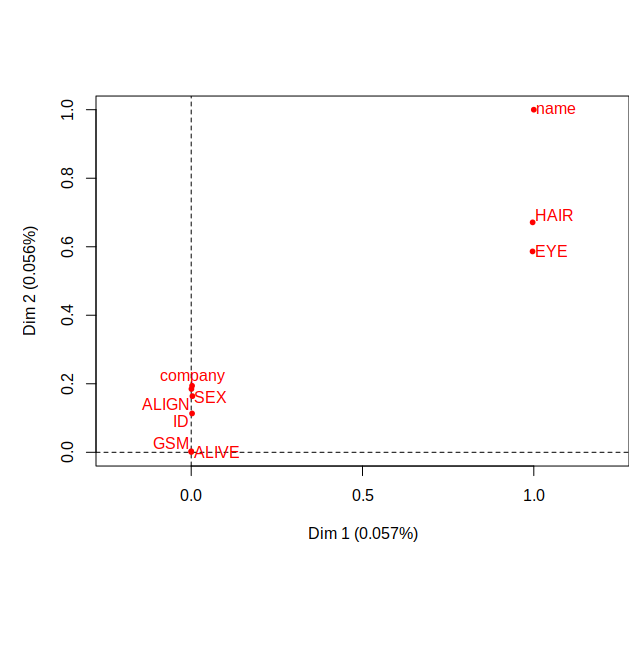
\includegraphics[scale=0.5]{img/MCA_01.png}
\end{center}

Which means that applying MCA to the totality of the dataset is not very reliable. Or, in other words, we cannot conclude there is a clear dependency between factors on the data analysed.

Since we know that this dataset contains \textbf{all} characters that have appeared in the series without taking into account if they are protagonists or just some people passing by and having only one speech bubble in the whole world, we have reduced the dataset to only those that have appeared at least more than 800 times. That is, we have focused on the real main characters.

This number has been chosen arbitrarily. First a value of at least 100 appearances had been chosen as criteria, but the number of variability explained in MCA was still very low, so it was increased even further.

 Below is a table that summarizes the number of appearances tried and the number of individuals resulted from it, as well as the maximum variability explained with 2 dimensions (the ones whith most \% of variability).


\begin{center}

\begin{tabular*}{0.8\textwidth}{l@{\extracolsep{\fill}}rr}
\textbf{\begin{tabular}[c]{@{}l@{}}Min.  \\ \# appearances\end{tabular}} & \textbf{\# Individuals} & \textbf{\begin{tabular}[c]{@{}r@{}}Variability \\ explained (\%)\end{tabular}} \\ \hline
- & 6799 & 0.1 \\
100 & 607 & 8.4 \\
500 & 99 & 13.73 \\
700 & 64 & 17.14 \\
\textbf{800} & \textbf{56} & \textbf{19.99} \\
1000 & 43 & 22.32 \\
1200 & 29 & 28.31
\end{tabular*}
\end{center}
\null
\vfill

Finally, it was determined that the more balanced subset was the one with 56 individuals by having as a criteria that each character had, at least, appeared 800 times throughout their series. This ended up with almost 20\% of variability explained.


Increasing the threshold more than what we have chosen would have meant increasing almost 10 points more on the variability explained at the cost of sacrificing too many individuals and being left with only 29, for example, in the last case.

So, using the 56 most popular characters in both universes as a dataset, the variability explained  when applying MCA in the dimensions found is:
\begin{center}
   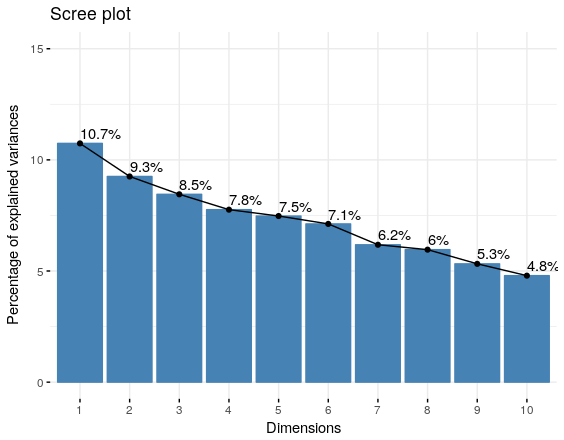
\includegraphics[scale=0.5]{img/MCA_scree_plot.png}
    \captionof{figure}{Scree plot of variability explained by each dimension.}
\end{center}

We can see that there is no dimension which clearly differentiates from the others by explaining twice or more of variability. So we chose to study the dataset using the first two dimensions as to plot the individuals and study their factors' structure.


\begin{figure}[!htb]
\hspace*{-1.3cm}
    \centering
    \begin{minipage}{.55\textwidth}
        \centering
        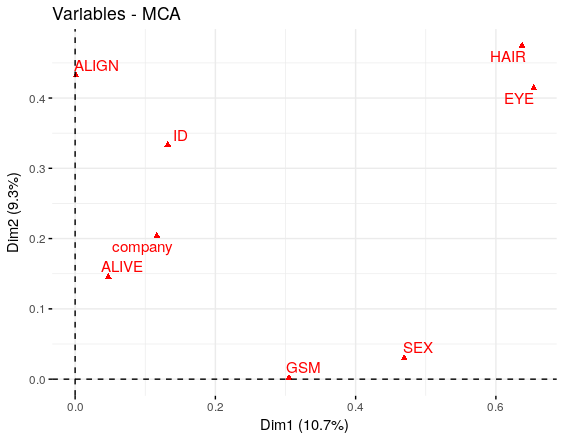
\includegraphics[width=\linewidth]{img/MCA_vars.png}
        \captionof{figure}{Variables MCA plot.}
    \end{minipage}%
     \begin{minipage}{.05\textwidth}
      \hfill
    \end{minipage}%
    \begin{minipage}{0.55\textwidth}
    \centering
        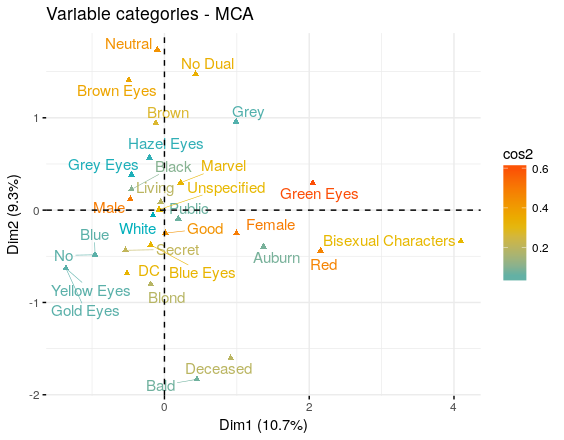
\includegraphics[width=\linewidth]{img/MCA_vars_cat_q.png}
        \captionof{figure}{Variables' categories MCA plot.}
    \end{minipage}
\end{figure}

\newpage
The variables MCA plot shown on the left figure shows the possible relations between the different variables.

For the most popular characters, there seems to be a correlation between the living status and the company they form part of. The same happens with their looks. It seems that there is a close relationship between the hair and eye color of a character. 
There also seem to be some degree of correlation between the character's alignment and their identity status, as well as the GSM and their sex.

In the right plot, we can see the possible relationship (or not) between categories from different variables.

For example, it seems that most of the deceased characters are bald. Or that most male characters seem to be alive.

There also seems that most characters with green eyes have red hair and are female.

However, we should not that both the bad and deceased categories are not of very good quality.
This quality is explained by the \textbf{$cos^2$} (squared cosine) variable. It measures how associated are the variable categories and the axis. When it is well associated this value tends to 1, while it tends to 0 when the opposite happens.

So, the greater the value of $cos^2$, the warmer the color as can be seen in the legend.
\begin{center}
   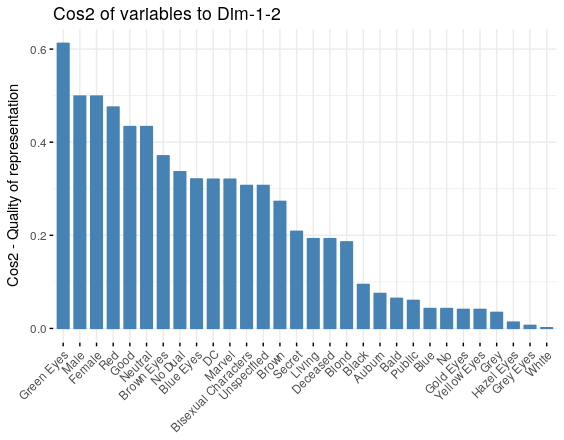
\includegraphics[scale=0.7]{img/cos2_quality.png}
\end{center}

As we can see in the plot above, the category of green eyes is well associated with the dimensions shown, as well as being male or female.


Apart from calculating the squared cosine, MCA also computes the level of contribution of a variable's category definition of the two selected dimensions.


\begin{center}
   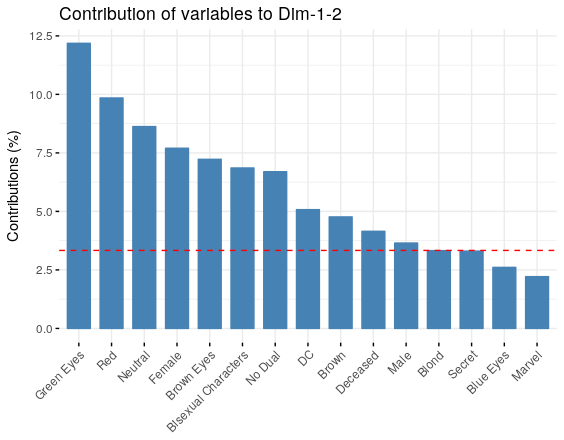
\includegraphics[scale=0.7]{img/contrib12.png}
\end{center}

In this case, the categories most contribution to the dimensions are again the eyes, red hair, neutral alignment and being female.



We can see the quality of data and their contribution to the two dimensions summarized in the following tables:

\begin{center}
  \begin{tabular*}{0.8\textwidth}{l@{\extracolsep{\fill}}rrlrr}
\multicolumn{6}{c}{\textbf{Quality of variables}} \\ \hline
\multicolumn{3}{c}{\textbf{Dim 1}} & \multicolumn{3}{c}{\textbf{Dim 2}} \\ \hline
\textbf{Variable} & \textbf{R2} & \multicolumn{1}{r|}{\textbf{p.value}} & \textbf{Variable} & \textbf{R2} & \textbf{p.value} \\ \hline
\textbf{EYE} & 0,654 & \multicolumn{1}{r|}{0} & \textbf{ALIGN} & 0,4321 & 0 \\
\textbf{SEX} & 0,4693 & \multicolumn{1}{r|}{0} & \textbf{ID} & 0,3335 & 0 \\
\textbf{HAIR} & 0,6374 & \multicolumn{1}{r|}{0} & \textbf{EYE} & 0,4141 & 0,0001 \\
\textbf{GSM} & 0,305 & \multicolumn{1}{r|}{0} & \textbf{HAIR} & 0,4744 & 0,0002 \\
\textbf{company} & 0,1165 & \multicolumn{1}{r|}{0,01} & \textbf{company} & 0,204 & 0,0005 \\
\textbf{ID} & 0,1322 & \multicolumn{1}{r|}{0,0234} & \textbf{ALIVE} & 0,1456 & 0,0037
\end{tabular*}

\end{center}

\begin{center}
\begin{tabular*}{0.85\textwidth}{l@{\extracolsep{\fill}}rrlrr}
\multicolumn{6}{c}{\textbf{Contribution to dimensions}} \\ \hline
\multicolumn{3}{c}{\textbf{Dim 1}} & \multicolumn{3}{c}{\textbf{Dim 2}} \\ \hline
\textbf{category} & \textbf{Estimate} & \multicolumn{1}{r|}{\textbf{p.value}} & \textbf{} & \textbf{Estimate} & \textbf{p.value} \\ \hline
\textbf{Green Eyes} & 1,2704 & \multicolumn{1}{r|}{0} & \textbf{Neutral} & 0,5013 & 0 \\
\textbf{Female} & 0,3986 & \multicolumn{1}{r|}{0} & \textbf{Brown Eyes} & 0,6373 & 0 \\
\textbf{Red} & 1,0573 & \multicolumn{1}{r|}{0} & \textbf{No Dual} & 0,584 & 0 \\
\textbf{Bisexual} & 1,1332 & \multicolumn{1}{r|}{0} & \textbf{Brown} & 0,5952 & 0 \\
\textbf{Marvel} & 0,2018 & \multicolumn{1}{r|}{0,01} & \textbf{Marvel} & 0,2478 & 0,0005 \\
\textbf{Auburn} & 0,6283 & \multicolumn{1}{r|}{0,0498} & \textbf{Living} & 0,4275 & 0,0037 \\
\textbf{Black} & -0,3633 & \multicolumn{1}{r|}{0,0397} & \textbf{Secret} & -0,3785 & 0,0321 \\
\textbf{DC} & -0,2018 & \multicolumn{1}{r|}{0,01} & \textbf{Deceased} & -0,4275 & 0,0037 \\
\textbf{Secret} & -0,3078 & \multicolumn{1}{r|}{0,0072} & \textbf{Blond} & -0,2858 & 0,0013 \\
\textbf{Unspecified} & -1,1332 & \multicolumn{1}{r|}{0} & \textbf{DC} & -0,2478 & 0,0005 \\
\textbf{Male} & -0,3986 & \multicolumn{1}{r|}{0} & \textbf{Blue Eyes} & -0,2637 & 0,0001 \\
 &  & \multicolumn{1}{r|}{} & \textbf{Good} & -0,5013 & 0
\end{tabular*}
  
\end{center}


\subsection{Grouping}

Having applied MCA we can also try to group each variables' categories and see if they tend to group by themselves or by contrary are scattered in no particular order.

\begin{center}
   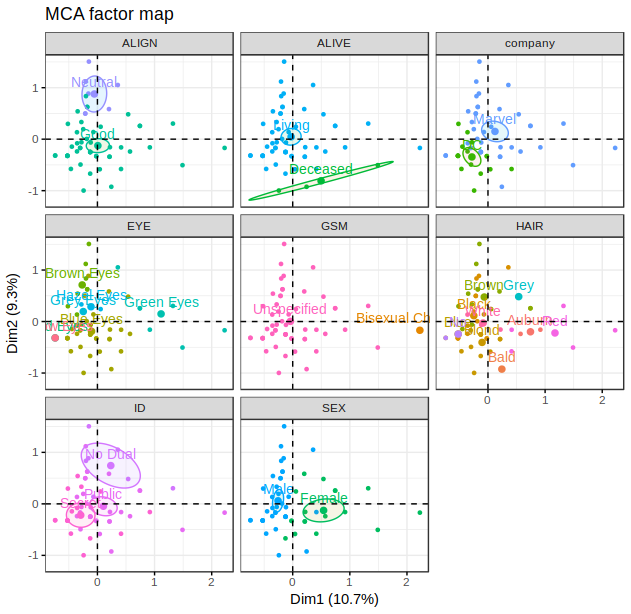
\includegraphics[scale=0.7]{img/MCA_all_factors.png}
\end{center}

We can observe that alignment, living status, company they are from, GSM (which is if they form part of a minority group such as bisexuality), identity and gender are clearly separated and even groupable, as shown with the ellipses.

However, hair and eye color are pretty mixed and non group discernable.


So this means that our MCA mapping is able to separate to a certain degree the good from the neutral, the living from the decease, the company they are from, their GSM, whether their identity is not dual, public or secret and between male and female characters.


\newpage
\section{Conclusions}
The conclusions to extract from this project are many.


First of all, \textbf{cleaning the dataset} strictly by removing all the rows which had some fields empty, leads to the reduction of the dataset by a 70\% in our case. The original dataset had too many empty fields, although we ended up still with a large dataset. It is important to have a quality dataset. In this case, although we reduced a lot the number of individuals to study, we still had a lot to work with (around 7000 individuals). But this may not be always the case when cleaning data and we could end up with very few individuals, not enough to be representative.

Secondly, it is clear that the target of the american comics has been a male population or, at least, \textbf{the comics have been male dominant}. However, these past decade there has been an\textbf{ increase} on the number of \textbf{female characters} which may be continued for the next years.

Thirdly, there is \textbf{twice the alive characters than deceased ones}. However, when looking at the subset of characters that have appeared most times, there is a \textbf{reticence on killing recurring characters}.

\textbf{Bad characters are also not very recurrent} since they haven't appeared in our \textit{main characters} subset of the dataset. Which induces us to think that there are many different antagonists.


Separately, we have seen that when applying MCA on this dataset \textbf{there really aren't many variables which are interconnected or dependent}, meaning that not many stereotypes have been found other than maybe hair and eyes color and even that structure is not very reliable, since only 20\% of the variability is explained.

However, I have found \textbf{MCA to be a pretty good technique to apply to qualitative data}, specially if one has already worked with quantitive or linear data applying \textbf{PCA}, which is really similar when interpreting the plots.

All in all, we cannot say that they produce characters with clearly dependent attributes or characteristics, since the variability explained in MCA when working with the whole dataset is lower than 1\%, and even when working with the characters that have appeared most throughout their series, only 20\% of information is explained using 2 dimensions in MCA.

Despite this, we have found that the american comics have been indeed focused on producing male characters although it seems they are trying to reduce the gap currently, and meanwhile there are mor bad male characters than good ones, females tend to be more \textit{good aligned} or neutral.

For \textbf{further studies} or work related to this field, it would be interesting to study more deeply each character in terms of  \textbf{personality traits, behaviour around other characters, speaking manners and socio-economic status}. This would lead to be able to see if even though there is no clear structure in physical components of a character, maybe they exist in the social level.


\newpage
\nocite{*}
\bibliographystyle{acm}
\bibliography{references} 

%https://github.com/fivethirtyeight/data/tree/master/comic-characters
% https://en.wikipedia.org/wiki/Multiple_correspondence_analysis
%https://fivethirtyeight.com/features/women-in-comic-books/
  %http://www.sthda.com/english/articles/31-principal-component-methods-in-r-practical-guide/114-mca-multiple-correspondence-analysis-in-r-essentials/
   
\end{document}
